\section{LoRa module}
In order to test the LoRa SX1278 module, one wrote a small program to test send and receive functions from LoRa module, with usage shown in figure \ref{fig:loratest}.

\begin{figure}[H]
	\centering	
	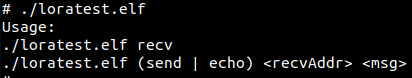
\includegraphics[width=0.6\textwidth]{13tests/lora/loratest}
	\caption{LoRa module test program.}
	\label{fig:loratest}
\end{figure}

Using two LoRa modules, one was connected to a Raspberry Pi in\linebreak
\verb|tomas-abreu|'s computer with local address defined as \verb|0xbb|, the other was connected to another Raspberry Pi in \verb|fernandes|'s computer with local address \verb|0xcc|.

One tested the read and send functions of the module, firstly by waiting for a message, as shown in figure \ref{fig:loratest_recv}.

\begin{figure}[H]
	\centering	
	\includegraphics[width=0.6\textwidth]{13tests/lora/BB_recv_wait}
	\caption{Test LoRa module: receive.}
	\label{fig:loratest_recv}
\end{figure}

In figure, device \verb|0xcc| sends the message \verb|"Hello from 0xCC"| to the device \verb|0xbb|.

\begin{figure}[H]%
	\centering
	\subfloat[\centering label	 1]{{\includegraphics[width=6.25cm]{13tests/lora/CC_send}}}%
	\qquad
	\subfloat[\centering label 2]{{\includegraphics[width=6.25cm]{13tests/lora/BB_recv}}}%
	\caption{2 Figures side by side}%
	\label{fig:example}%
\end{figure}



begun by analyzing the signals sent 


\section{TSL2581}

\section{PWM control}

\section{Motion Detector}